\documentclass[UTF8,a4paper,12pt]{ctexart}  % Latex 去掉上面的语句,加上本语句
\usepackage{xeCJK}

\IfFileExists{C:/Windows/Fonts/AdobeSongStd-Light.otf}{
  \setCJKmainfont[BoldFont=AdobeHeitiStd-Regular]{AdobeSongStd-Light}}
{\setCJKmainfont[BoldFont=SimHei]{SimSun}}

\IfFileExists{C:/Windows/Fonts/AdobeSongStd-Light.otf}{
  \setCJKfamilyfont{song}{AdobeSongStd-Light}}{
  \setCJKfamilyfont{song}{SimSun.ttc}}

\IfFileExists{C:/Windows/Fonts/AdobeHeitiStd-Regular.otf}{
  \setCJKfamilyfont{hei}{AdobeHeitiStd-Regular}}{
  \setCJKfamilyfont{hei}{SimHei.ttf}}

\IfFileExists{C:/Windows/Fonts/AdobeKaitiStd-Regular.otf}{
  \setCJKfamilyfont{kai}{AdobeKaitiStd-Regular}}{
  \setCJKfamilyfont{kai}{SimKai.ttf}}

\IfFileExists{C:/Windows/Fonts/AdobeFangsongStd-Regular.otf}{
  \setCJKfamilyfont{fs}{AdobeFangsongStd-Regular}}{
  \setCJKfamilyfont{fs}{SimFang.ttf}}

% \setCJKfamilyfont{fs}{Sun Yat-sen Hsingshu}


\renewcommand{\contentsname}{\centerline{\textcolor{violet}{目 \ \ 录}}}    % 将Contents改为目录
\renewcommand{\abstractname}{摘 \ \ 要}      % 将Abstract改为摘要
\renewcommand{\refname}{参考文献}            % 将Reference改为参考文献
\renewcommand\tablename{表}
\renewcommand\figurename{图}
\renewcommand{\today}{\number\year 年 \number\month 月 \number\day 日}

\usepackage[dvipsnames]{xcolor}
\PassOptionsToPackage{colorlinks=true,citecolor=blue, urlcolor=blue, linkcolor=violet, bookmarksdepth=4,bookmarksnumbered=true,bookmarksopen=true,bookmarksopenlevel=2}{hyperref}

\usepackage{lscape}
\usepackage{indentfirst}
\usepackage{textcomp}                      % provide many text symbols
\usepackage{setspace}                      % 各种间距设置

% ---------------------------------Table------------------------------
\usepackage{longtable}
\usepackage{booktabs}
\usepackage{array}                         % 提供表格中每一列的宽度及位置支持
\usepackage{rotating}
\usepackage{multirow}
\usepackage{wrapfig}
\usepackage{colortbl}
\usepackage{pdflscape}
\usepackage{tabu}
\usepackage{threeparttable}
\usepackage{threeparttablex}
\usepackage[normalem]{ulem}
\usepackage{makecell}
\newcolumntype{L}[1]{>{\raggedright\let\newline\\\arraybackslash\hspace{0pt}}m{#1}}
\newcolumntype{C}[1]{>{\centering\let\newline\\\arraybackslash\hspace{0pt}}m{#1}}
\newcolumntype{R}[1]{>{\raggedleft\let\newline\\\arraybackslash\hspace{0pt}}m{#1}}

%% 参考文献
\usepackage{gbt7714}
\usepackage{natbib}
\setlength{\bibsep}{0.5pt}


\usepackage[utf8]{inputenc}
% \usepackage[T1]{fontenc} % [T1] 主要支持东欧等国家重音符 , 与下面 consolas 冲突
\usepackage{fontenc}
\usepackage{fixltx2e}
\usepackage{graphicx}
\usepackage{float}
\usepackage{wrapfig}
\usepackage{soul}
\usepackage{textcomp}

\newcommand\hmmax{0} %% 防止Too many math alphabets used in version normal.
\newcommand\bmmax{0} %% 防止Too many math alphabets used in version normal.

\usepackage{lmodern,bm}   % 必需出现在amsmath等包前面,否则会出错
\usepackage{amsmath}
\usepackage{marvosym}
\usepackage{wasysym}
\usepackage{latexsym}
\usepackage{amssymb}
\usepackage{hyperref}
\usepackage{listings}
\usepackage{tikz}

\setmonofont{Consolas} % listings 中支持 consolas 字体,必需配合上面\usepackage{fontenc} 中不出现[T1]才可以

\lstset{numbers=left, numberstyle=\ttfamily\tiny\color{Gray}, stepnumber=1, numbersep=8pt,
  frame=leftline,
  framexleftmargin=0mm,
  rulecolor=\color{CadetBlue},
  backgroundcolor=\color{Periwinkle!20},
  stringstyle=\color{CadetBlue},
  flexiblecolumns=false,
  aboveskip=5pt,
  belowskip=0pt,
  language=R,
  basicstyle=\ttfamily\footnotesize,
  columns=flexible,
  keepspaces=true,
  breaklines=true,
  extendedchars=true,
  texcl=false,  % 必须设置为false设置为true的时候 R 代码中不能含有多个注释符号 #
  upquote=true,
  showstringspaces=false,
  keywordstyle=\bfseries,
  keywordstyle=\color{Purple},
  xleftmargin=20pt,
  xrightmargin=10pt,
  morecomment=[s]{\#}{\#},
  commentstyle=\color{OliveGreen!60}\scriptsize,
  tabsize=4}

\tolerance=1000

%======================== 根据选项设置代码处理方式 RMARKDOWN 中独有=============

\providecommand{\tightlist}{\setlength{\itemsep}{0pt}\setlength{\parskip}{0pt}}
\newcommand{\passthrough}[1]{\lstset{mathescape=false}#1\lstset{mathescape=true}}

\author{\CJKfamily{kai} 金 \enspace 林 \\ \CJKfamily{kai} 中南财经政法大学统计系 \\ jinlin82@gmail.com}
% ------------------------Chapter Section Title-------------------------
%--- 英文期刊标题 -----
\usepackage{titlesec}
\titleformat{\section}{\large\bfseries}{\thesection}{1em}{}
\titleformat{\subsection}{\normalsize\bfseries}{\thesubsection}{0.5em}{}
\titlespacing{\section}{0pt}{1ex plus 1ex minus .2ex}{1ex plus 1ex minus .2ex}
\titlespacing{\subsection}{0pt}{0.5ex plus 1ex minus .2ex}{0.5ex plus 1ex minus .2ex}
%--- 中文期刊标题 -----
% \CTEXsetup[name={,、}, number={\chinese{section}}, aftername={},
% format={\large \heiti }, indent={24pt},
% beforeskip={1ex plus 1ex minus .2ex},
% afterskip={1ex plus 1ex minus .2ex}]
% {section}
% \CTEXsetup[name={(,)}, number={\chinese{subsection}}, aftername={},
% format={\normalsize \bfseries \songti}, indent={\parindent},
% beforeskip={0.5ex plus 1ex minus .2ex},
% afterskip={0.5ex plus 1ex minus .2ex}]
% {subsection}
% \CTEXsetup[name={,.}, number={\arabic{subsubsection}},
% aftername={}, format={\normalsize \bfseries \songti},indent={\parindent},
% beforeskip={0ex plus 1ex minus .2ex},
% afterskip={0.2ex plus 1ex minus .2ex}]
% {subsubsection}

% ------------------------Figure and Table Caption---------------------
%\makeatletter                        % 图表标题格式设置
%\renewcommand{\fnum@table}[1]{\small \bfseries\textcolor{Violet}{\tablename\thetable~~}}
%\renewcommand{\fnum@figure}[1]{\small \CJKfamily{hei} \textcolor{Violet}{\figurename\thefigure~~}}
%\makeatother

\usepackage[skip=0pt, labelsep=quad, font={small, bf}, labelfont={color={Violet}}]{caption}

\renewcommand{\thefigure}{\arabic{figure}}
\renewcommand{\thetable}{\arabic{table}}
\newcommand{\HRule}{\rule{\linewidth}{0.5mm}}

\usepackage[top=2cm,bottom=2cm,left=3cm,right=3cm]{geometry}
\sloppy
\linespread{1.2}                    % 设置行距
\setlength{\parindent}{24pt}        % 段落缩进
\setlength{\parskip}{1ex plus 0.5ex minus 0.2ex}
\pagestyle {plain}                  % 去掉页眉
\setcounter{secnumdepth}{4}

%%% Change title format to be more compact
\usepackage{titling}

% Create subtitle command for use in maketitle
\newcommand{\subtitle}[1]{
  \posttitle{
    \begin{center}\large#1\end{center}
    }
}

\setlength{\droptitle}{-2em}

  \title{}
  \pretitle{\vspace{\droptitle}}
  \posttitle{}


  \author{}
  \preauthor{}\postauthor{}

  \date{}
  \predate{}\postdate{}


\begin{document}







\hypertarget{section}{%
\section{引言}\label{section}}

贵金属市场是一个既具备商品属性,又兼备金融属性的市场,作为金融投资商品,不仅对大宗商品交易市场有影响,甚至影响全球经济的稳定性。黄金等贵金属由于其稀缺性、价值稳定性及交易便利性受到投资者喜爱,其交易活动也日趋活跃。与股票债券不同,黄金现货即期合约采用T+0交易方式,可随时建仓,也可随时平仓;黄金现货延期交收合约采用T+D交易方式,交易方式为分期付款,交易方并不被要求必须当日交割,其允许延期交割,且无限期;如若夜间国际金价发生巨大波动,夜盘交易有利于回避其现象对国内不利的影响,
增加了投资机会;保证金交易,提高资金利用率\citep{郭凡礼2015}。

2019年12月底新冠病毒在中国被发现,即使各地政府极力防护,但最终也演变为蔓延全世界的重大事件,世界经济处于自2008年全球金融危机以来最不稳定的状态,不可避免的造成全球经济的``停摆''。2020年3月,我国疫情接近尾声,而新冠肺炎在欧美国家大面积爆发,美股在十天内发生了四次熔断。面对通货膨胀压力,不断加剧的金融市场风险,投资者对资金的避险需求不断提高,贵金属市场尤其是黄金市场的保值增值能力,引起了投资者的关注。金融市场动荡下,贵金属市场的走势如何,贵金属产品的波动性会有何特征值得探究。

然而,随着现代金融市场的快速发展,市场波动变化相比与以往更难把握,高频数据在对市场波动等相关信息的呈现远远超过传统的低频数据。科技水平的提高使得高频数据的获取成为可能,如果能充分利用数据自身包含的信息,将高频数据与易于估计的模型相结合,就可以提高对产品波动性的估计精度。

本文以黄金代表贵金属现货市场,选取2019年7月1日至2020年12月31日黄金T+D高频价格数据作为研究对象,对贵金属产品的波动性进行研究。通常,金融时间序列表现为尖峰厚尾的特征,其收益率一般不服从正态分布,故本文采用Realized~GARCH模型对残差服从正态分布,t分布,偏t分布、广义双曲线分布等对黄金的收益率序列进行拟合,根据极大似然函数值和风险价值预测选出拟合效果较好的分布,并对其波动特征进行分析。

\hypertarget{section-1}{%
\section{国内外文献综述}\label{section-1}}

\hypertarget{section-2}{%
\subsection{贵金属市场波动性研究综述}\label{section-2}}

波动性意味着价格在某一时间间隔所发生的变化,与投资者的收益息息相关。之前对于贵金属市场波动性的研究,学者采取了不同的模型及研究方法。林新丹(2014)通过对我国黄金和白银期货价格的相关性研究结果说明高频数据更有助于对黄金、白银等贵金属价格的预测,2013
年黄金大跌对白银市场造成了巨大的冲击,影响程度达到90\%以上\citep{林新丹2014}。杨胜刚等
(2019)对伦敦金属交易所的四种贵金属(黄金、白银、铂金和钯金)基于time-varying AR模型构建有效性程度指标对适应性市场假说(AMH)进行实证研究,发现黄金市场有效性程度指标的均值和波动幅度相对最小,而钯金市场的均值和波动幅度则相对最大\citep{杨胜刚2019}。

\hypertarget{section-3}{%
\subsection{已实现波动率研究综述}\label{section-3}}

在现代金融市场中,波动率是一种可以反映金融资产价格变化的统计度量,准确度量和预测金融资产波动率,在金融资产定价,金融风险控制等决策中是不可或缺的一步。传统对金融市场的波动率研究大多基于日、周、月等低频交易数据,如GARCH类和SV类模型。随着信息技术的不断提高,高频数据的易获取使得人们对波动率的研究更进一步。

Merton(1980)在研究市场预期收益时首次提出已实现波动率的概念,将一个时间段划分为多个子时间段区间,用多个子时间段的收益率平方和估计该时间段的收益率方差
\citep{MertonRobert1980}。已实现波动率概念提出以后,由于当时的技术限制,划分数据子区间还不能实现,无法真正应用到实践中。Andersen和Bollerslev等人(1998)首次将高频数据应用于波动率的测度上,提出已实现波动率(RV,Realized Volatility)的估计计算方法
\citep{TimBollerslev},与传统的根据历史日间交易数据估计波动率不同,这种方法直接利用``日内收益平方和''估计波动率,证明了当抽样频率非常大时,已实现波动是积分波动的一致估计量。

\hypertarget{realized-garch}{%
\subsection{Realized GARCH类模型文献综述}\label{realized-garch}}

已实现波动率是把高频数据应用到波动率领域,使得金融资产的波动率能够直观表示。
Hansen等人(2012)提出了Realized GARCH 模型,将已实现波动率与GARCH(广义自回归条件异方差模型)结合,通过一个测量方程连接条件方差和已实现波动率,并在方程这种加入杠杆函数体现非对称效应,把已实现波动率作为条件方差的估计,实现收益率,波动率和已实现测度的联合建模,和传统GARCH类模型相比,Realized GARCH 模型提高了拟合能力和波动性的预测能力\citep{Hansen2012}。后来很多学者将Realized GARCH模型进行了各种各样的延伸,并广泛应用于一些金融实证研究中。下面主要对一元Realized GARCH模型的发展、应用等进行叙述。

由于金融时间序列往往不具备正态分布的特征,Watanbe(2012)将Hansen(2012)提出的残差服从正态分布的Realized GARCH 模型扩展为残差服从t分布,偏t分布的Realized GARCH 模型,并对基于这三种分布下的Realized GARCH 模型预测VaR和ES进行对比研究
\citep{Watanabe2012}。Huang等人(2016)对S\&P500指数期权进行实证研究,表明基于Realized
GARCH 模型算出的定价误差小于传统模型\citep{Huang2016b}。

\hypertarget{section-4}{%
\subsection{文献评述}\label{section-4}}

从贵金属市场研究文献看,国内学者对贵金属的研究主要集中在黄金、白银、铂金上,更为常见的是集中在对黄金市场的相关分析上。因此,本文选取黄金代表贵金属市场进行波动性研究。

已实现波动测度是基于高频数据计算的,阅读文献可知Realized GARCH类模型有两个基本条件:高频数据的获取以及已实现波动率的计算及最优选择。高频数据能够反映更多信息,相比于低频日数据,基于高频数据对波动率等的拟合和预测性能更佳。对于一元Realized
GARCH模型,针对金融时间序列尖峰厚尾的特性,将Realized GARCH模型残差分布从正态分布扩展到t分布,偏t分布、广义双曲线分布等,通过比较不同分布下的预测效果选择最优模型。

\hypertarget{realized-garch-1}{%
\section{已实现波动率及Realized Garch类模型基础介绍}\label{realized-garch-1}}

\hypertarget{section-5}{%
\subsection{已实现波动率}\label{section-5}}

已实现波动率是基于高频数据度量的金融资产波动率。假定不考虑由买卖价差、闭市效应、非同步交易等因素,且没有发生跳跃,按照 Andersen和Bollerslev(1998)对已实现波动率的计量,已实现的波动率RV是计算期第\(t\)日观测到的收益率的平方和,每日交易被分割为\(M\)
段,当\(M\)趋向于无穷大时
\protect\hypertarget{eq:RV}{}{\begin{equation}RV_t=\sum_{i=1}^Mr_{t,i}^2\label{eq:RV}\end{equation}}
  \(r_{t,i}\)为金融资产或者资产组合在第 \(t\)交易日内的第 \(i\) 个间隔的日内对数收益率,\(lnP_{t,i}\)表示金融资产或者资产组合在第\(t\) 个交易日内的第 \(i\) 个间隔的日内对数价格,\(T\) 表示计数天数,\(M\)表示每天的时间间隔为M,与采样频率有关\citep{TimBollerslev}。

\hypertarget{realized-garch-2}{%
\subsection{Realized Garch模型}\label{realized-garch-2}}

普通的GARCH类模型一般是通过每日收益获得相应的波动率结果,但是波动率是通过滞后多阶的条件方差计算得到的,所以当收益情况波动剧烈时,GARCH类模型较难把所有信息有效利用。Hansen等(2012)提出Realized Garch模型,该模型用波动率的已实现测度代替对未来波动率进行建模\citep{Hansen2012}。

根据Hansen等(2012)的研究结果,Realized Garch模型在一阶下的估计效果已经相当不错,所以本文主要采用Realized GARCH(1,1)模型进行实证研究,该模型具体形式为
\protect\hypertarget{eq:rg1}{}{\begin{equation}
\begin{cases}
r_{t}=\sqrt{h_{t}} z_{t},z_t\sim N(0,1)\\
\ln h_{t}=\omega+\beta \ln h_{t-1}+\alpha \ln x_{t-1}\\
ln x_{t}=\xi+\varphi \ln h_{t}+\tau\left(\mathrm{z}_{t}\right)+u_{t},u_{t} \sim iid  \left(0, \sigma_{u}^{2}\right)
\end{cases}
\label{eq:rg1}\end{equation}}
  模型的三个等式分别为收益方程、GARCH方程和测量方程。\(r_t\)是第\(t\)
日的日收益率,\(h_t=var(r_t|F_{t-1})\)表示收益率的条件方差,\(x_t\)表示第\(t\)日波动率的已实现测度,本文使用RV作为已实现波动率的估计。\(z_t\)是收益率的标准随机误差项,残差项 \(u_{t} \sim iid\left(0, \sigma_{u}^{2}\right)\),残差项可服从正态分布、t分布、偏t分布、广义双曲线分布等。\(z_t\)与\(u_{t}\)相互独立。测量方程将\(h_t\)和\(x_t\)联系起来。在
Realized GARCH 模型中\(h_t\)是\(h_{t-1}\)和\(x_t\)的函数。

考虑到收益率冲击对波动率具有一定的非对称影响,本文在测量方程中引入了杠杆函数
\(\tau(z_t)\),Hansen等(2012)人将\(\tau(z_t)\)设定为以下二次形式\protect\hypertarget{eq:tau}{}{\begin{equation}\tau(z_t)=\tau_1z_t+\tau_2(z_t^2-1)\label{eq:tau}\end{equation}}
  杠杆函数描述了Realized GARCH 模型的信息冲击曲线,表明过去时刻的收益率在大小和方向上同时都影响着波动率,即正的价格扰动对波动的影响和负的价格扰动对波动率产生的影响在大小和方向上都不一致的。

\hypertarget{realized-garch-3}{%
\section{基于Realized Garch模型对贵金属市场波动性分析}\label{realized-garch-3}}

\hypertarget{section-6}{%
\subsection{贵金属市场对象选取和数据预处理}\label{section-6}}

\hypertarget{section-7}{%
\subsubsection{研究对象的选取}\label{section-7}}

贵金属主要包含金、银和铂族金属等金属元素,我国贵金属的现货交易主要在上海黄金交易所进行。通过计算上海黄金交易所中近2年产品月成交量占比可发现,黄金延期
Au(T+D)的月成交量占比基本在95\%以上,且其上市时间也相对较久,因此本文将选择黄金延期Au(T+D)合约作为研究对象,以代表贵金属现货市场进行研究。

现货交易分日市交易和夜市交易,一般情况(即非国家法定节假日)下,日间交易时间为星期一到星期五的09:00-15:30,夜市交易时间为星期一到星期五的20:00-02:30。所以不能按传统的交易日来看,即当天发生的交易为一个交易日来进行研究。对本文研究的对象
Au(T+D)来说,当交易日非国家法定节假日时,前日20:00对应交易日的开盘价,当日15:30
对应交易日收盘价;当交易日为国家法定节假日时,后日9:00为开盘时间,15:30为收盘时间。

\hypertarget{section-8}{%
\subsubsection{数据预处理}\label{section-8}}

本文选择5分钟的频率作为高频数据的抽样频率,选取Au(T+D)的5分钟交易数据,样本区间为2019年7月1日晚八点至2020年12月31日下午三点半,数据源自东方财富旗下的Choice金融终端数据库。

由于黄金含有夜市交易和日市交易,因此将数据分为两类处理。国家法定节假日后的第一天交易数据从当日9:00至15:30的交易形成,每天有80个时间间隔,其他交易日交易时间为前一日20:00至当日02:30,9:00至15:30,每天有158个时间间隔。由于开盘价是集中竞价\footnote{集中竞价有利于提高交易效率,降低交易成本,减少交易纠纷。}的结果,所以剔除9:00,20:00的数据。将数据分为两组,第一组为2019年7月1日至2020年6月30日,作为样本内数据用于拟合模型,第二组为2020年7月1日至2020年12月31日,作为样本外数据,用于对比检验模型效果。对于交易数据的处理,剔除当天停牌或者价格几乎不变化的交易日。经过数据处理后,Au(T+D)有367个交易日,共有56160个5分钟的高频数据。

考虑到隔夜价格的影响,收益率计算方式将依据``当日收盘价-前一日收盘价''。设\(t\)为任意一个特定的交易日,\(p_{t,j}\)表示第\(t\)日的第\(j\)个区间的收盘价,在第\(t\)个交易日中,第\(j\)个区间的对数收益率为\protect\hypertarget{eq:rt}{}{\begin{equation}r_{t, j}=\ln p_{t, j}-\ln p_{t, j-1}\label{eq:rt}\end{equation}}

\hypertarget{section-9}{%
\subsection{贵金属高频数据描述性分析及检验}\label{section-9}}

\hypertarget{section-10}{%
\subsubsection{描述性统计分析}\label{section-10}}

本节首先根据式(\ref{eq:rt})计算出Au(T+D)2019年7月1日至2020年12月31日的的每日收益率,共367个收益率数据。然后根据样本区间每个交易日的以5min为时间间隔的收盘价分别计算出Au(T+D)的高频日内收益率,进而计算相关已实现测度估计量,本文采用已实现测度估计量RV。考虑到计算出来的收益率过小,为了方便研究,将收益率结果扩大100倍。

\hypertarget{section-11}{%
\paragraph{序列图}\label{section-11}}

Au(T+D)收盘价和收益率时序图如图\ref{fig:Aurtplot}所示,从Au(T+D)的日收盘价时序图中可以看出,Au(T+D)价格整体呈上升趋势,但期间也有较大的波动。在收益率时序图中,收益率围绕着零上下波动,波动的幅度与收盘价的涨幅情况基本一致,2020年3-4月和
8-9月收益率波动幅度较大,具有明显的``波动性聚集''特征。从2020年3月开始,国外疫情逐渐严重、风险资产也愈跌愈烈、市场整体消极,黄金的避险属性由此凸显,出现价格上涨和收益率大幅度波动的情况。2020年8月,各国开始陆陆续续公布新冠疫苗的进展,市场有所回暖,但也在一定程度上造成黄金的下跌,其对应的收益率也波动剧烈。

\begin{figure}[H]

{\centering 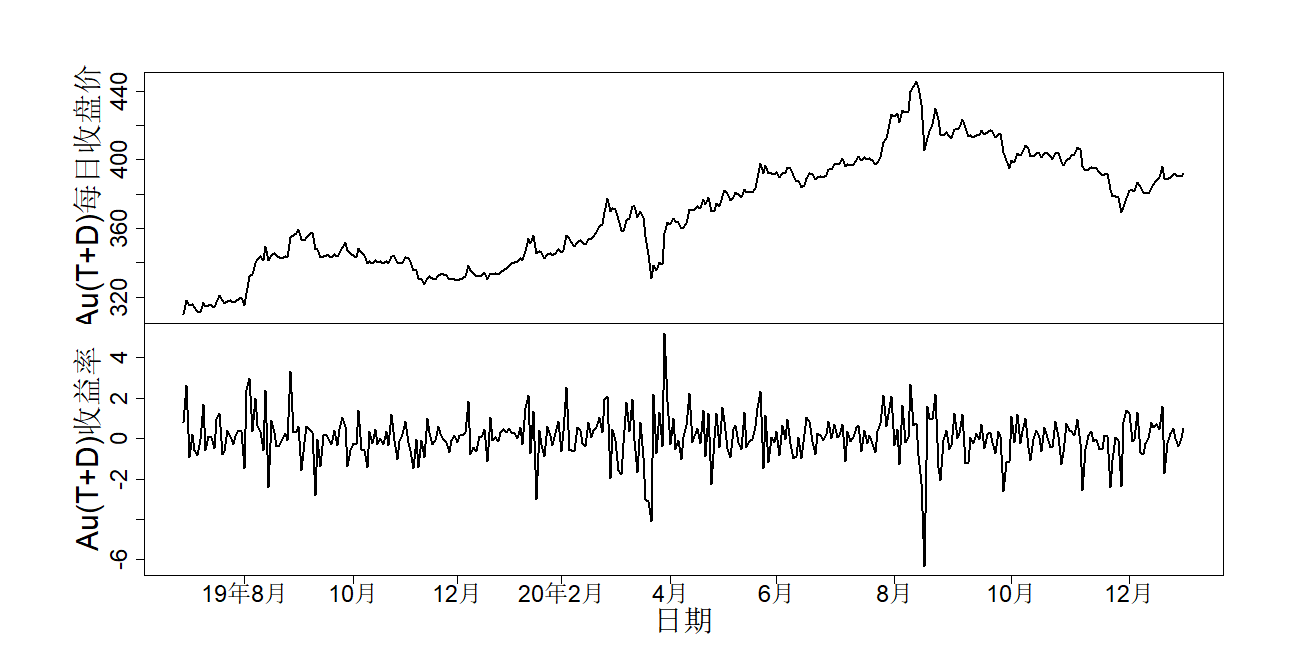
\includegraphics[width=0.95\linewidth]{03-estimation-lytfinal_files/figure-latex/Aurtplot-1} 

}

\caption{Au(T+D)收盘价和收益率序列时序图}\label{fig:Aurtplot}
\end{figure}

\hypertarget{section-12}{%
\paragraph{基本统计特征}\label{section-12}}

表\ref{tab:Aucharacteristics}列出了Au(T+D)对数收益率序列\(r_t\)和已实现测度RV序列的统计特征。可以明显看出,\(r_t\)和\(RV\)序列的峰度分别为4.853和33.296,均大于3,可认为它们都具有高峰厚尾的特征,Au收益率序列\(r_t\)偏度小于0,说明其左偏,波动率估计量\(RV\)偏度均大于0,具有右偏特征,且峰度较大。两个序列的J-B统计量\footnote{J-B统计量又名Jarque-Bera统计量,可以用来检验观测对象是否服从正态分布。}均较大,表现了显著不服从于正态分布的特点。

\begin{longtable}[t]{lccccccc}
\caption{\label{tab:Aucharacteristics}Au(T+D)收益率和已实现测度统计特征}\\
\toprule
  & 均值 & 最小值 & 最大值 & 标准差 & 偏度 & 峰度 & JB统计量\\
\midrule
\endfirsthead
\caption[]{\label{tab:Aucharacteristics}Au(T+D)收益率和已实现测度统计特征 (续)}\\
\toprule
  & 均值 & 最小值 & 最大值 & 标准差 & 偏度 & 峰度 & JB统计量\\
\midrule
\endhead

\endfoot
\bottomrule
\endlastfoot
Au\_rt & 0.0654 & -6.337 & 5.219 & 1.096 & -0.4433 & 4.853 & 378.7\\
Au\_RV & 0.7717 & 0.047 & 10.819 & 1.163 & 5.1468 & 33.296 & 18789.3\\*
\end{longtable}

\hypertarget{section-13}{%
\subsubsection{基本检验}\label{section-13}}

\hypertarget{section-14}{%
\paragraph{平稳性检验}\label{section-14}}

为保证实证结果的可靠性,在进行实证分析之前首先要对收益率序列进行平稳性检验。本文采用ADF检验法,检验结果如表\ref{tab:Au-adf}所示。

\begin{longtable}[t]{lcc}
\caption{\label{tab:Au-adf}Au(T+D)收益率序列平稳性检验}\\
\toprule
  & 检验统计量 & P值\\
\midrule
ADF检验 & -8.458 & 0.0001\\
\bottomrule
\end{longtable}

通过表\ref{tab:Au-adf}的平稳性检验结果可以看到,Au(T+D)收益率序列\(r_t\)的ADF检验的p值远小于显著性水平0.01,拒绝原假设,因此可以认为Au(T+D)收益率\(r_t\)序列是平稳的。

\hypertarget{section-15}{%
\paragraph{白噪声检验}\label{section-15}}

对Au(T+D)的收益率序列进行白噪声检验,这里分别运用(偏)自相关系数图和
Ljung-Box Q 统计量对Au(T+D)的收益率序列进行分析。

\begin{figure}[H]

{\centering 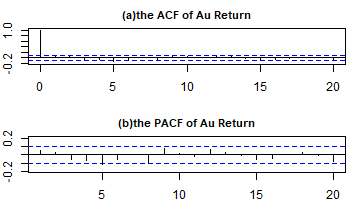
\includegraphics[width=0.95\linewidth]{03-estimation-lytfinal_files/figure-latex/acf-pacf-1} 

}

\caption{收益率自相关图和偏自相关图}\label{fig:acf-pacf}
\end{figure}

图\ref{fig:acf-pacf}显示了Au(T+D)的收益率序列\(r_t\)的自相关图和偏自相关图,从图中可以看出,滞后阶数为20阶以内下,自相关系数均未超出 95\%置信区间,表明序列不具有自相关性;偏自相关系数也均未超出95\%置信区间,表明序列不具有偏自相关性。

\begin{longtable}[t]{lccc}
\caption{\label{tab:Au-LB}Au(T+D)收益率序列纯随机性检验}\\
\toprule
  & LB统计量 & 延迟阶数 & P值\\
\midrule
纯随机性检验 & 14.62 & 10 & 0.1464\\
\bottomrule
\end{longtable}

Ljung-Box检验是用于检验给定时间序列是否存在滞后相关性的一种检验方法,原假设为序列为白噪声序列。通过表\ref{tab:Au-LB}的平稳性检验结果可以看到,Au(T+D)收益率序列Ljung-Box Q统计量的值为 14.6229 ,对应p值为0.1464 ,大于显著性水平0.05,故Au(T+D)收益率序列为白噪声序列,不具有相关性。

综合之前的平稳性检验,可以判断对数收益率序列\(r_t\)是一个平稳白噪声序列,不用构建ARMA模型。

\hypertarget{section-16}{%
\paragraph{残差平方序列异方差性检验}\label{section-16}}

\begin{figure}[H]

{\centering 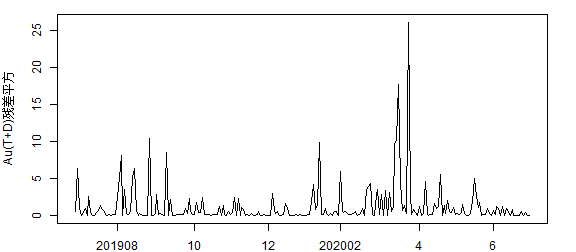
\includegraphics[width=0.95\linewidth]{03-estimation-lytfinal_files/figure-latex/resi2-1} 

}

\caption{收益率残差平方时序图}\label{fig:resi2}
\end{figure}

经标准化后得到的残差平方时序图如图\ref{fig:resi2}所示,从图中可以看出,对于
Au(T+D)收益率去均值化后的残差依然有较显著的``波动性聚集''特征,这说明收益率序列可能存在异方差现象,需要进行异方差性检验。本文运用ARCH检验方法中的LM检验。

\begin{longtable}[t]{lccc}
\caption{\label{tab:Au-ARCH}Au(T+D)残差平方序列ARCH检验}\\
\toprule
  & LM检验统计量 & 自由度 & P值\\
\midrule
ARCH LM-检验 & 28.2 & 5 & 0\\
\bottomrule
\end{longtable}

ARCH效应的存在会导致估计的有效性降低,其原假设为:残差序列中直到p阶都不存在ARCH
效应。对标准化后的残差平方进行ARCH效应检验,检验结果如表\ref{tab:Au-ARCH}所示。
Au(T+D)的LM统计量的值为28.2,对应的P值为0.0000,在0.05的显著性水平上拒绝残差独立的原假设,表明标准化后的残差平方存在ARCH效应。因此需对Au(T+D)收益率的残差拟合
GARCH模型,以消除ARCH效应。

\hypertarget{realized-garch-4}{%
\subsection{基于Realized Garch模型对黄金的波动率建模}\label{realized-garch-4}}

\hypertarget{realized-garch-5}{%
\subsubsection{不同分布下Realized Garch模型参数估计}\label{realized-garch-5}}

前文的分析指出Au(T+D)收益率序列具有波动特点。相较于普通的GARCH类模型而言,基于高频数据构建的Realized Garch模型更能真实的反映序列的波动性,且低阶 GARCH类模型的拟合效果较好,且在精度方面不存在太大的差距,结果可靠。因此本文选择基于5分钟的高频收益率对Au(T+D)进行建模,选择已实现方差RV作为已实现测度,将Realized GARCH的阶数定为(1,1)。

在分布类型的选取方面,由前文的分析可知,Au(T+D)收益率序列和已实现测度RV表现为偏态和尖峰厚尾的特征,表现为非正态分布。为了准确地描述序列的厚尾性,分布类型依次选取正态分布(N)、对肥尾特点刻画比较灵活的学生 t 分布(T)、偏t分布
(ST)和广义双曲线分布(GH)。选用R软件的rugarch包进行Realized GARCH模型的构建。

\begin{ThreePartTable}
\begin{TableNotes}[para]
\small
\item \textit{注:} 
\item 每个参数估计结果的第一行为参数值大小,第二行为每个估计结果的p值。
\end{TableNotes}
\begin{longtabu} to \linewidth {>{\centering\arraybackslash}p{1.8cm}>{\centering\arraybackslash}p{1.1cm}>{\centering\arraybackslash}p{1.1cm}>{\centering\arraybackslash}p{1.1cm}>{\centering\arraybackslash}p{1.1cm}>{\centering\arraybackslash}p{1.1cm}>{\centering\arraybackslash}p{1.1cm}>{\centering\arraybackslash}p{1.1cm}>{\centering\arraybackslash}p{1.1cm}>{\centering\arraybackslash}p{1.1cm}}
\caption{\label{tab:Au-estimate}Au(T+D)不同模型参数估计结果}\\
\toprule
模型形式 & $\omega$ & $\alpha$ & $\beta$ & $\tau_1$ & $\tau_2$ & $\delta$ & $\lambda$ & $\xi$ & $\pi$\\
\midrule
\endfirsthead
\caption[]{\label{tab:Au-estimate}Au(T+D)不同模型参数估计结果 (续)}\\
\toprule
模型形式 & $\omega$ & $\alpha$ & $\beta$ & $\tau_1$ & $\tau_2$ & $\delta$ & $\lambda$ & $\xi$ & $\pi$\\
\midrule
\endhead

\endfoot
\bottomrule
\insertTableNotes
\endlastfoot
N & 0.373 & 0.435 & 0.339 & -0.221 & 0.225 & 1.11 & 0.563 & -0.822 & 0.819\\
 & 0.000 & 0.000 & 0.002 & 0.000 & 0.000 & 0.00 & 0.000 & 0.000 & -\\
T & 0.539 & 0.503 & 0.304 & -0.244 & 0.261 & 1.02 & 0.562 & -0.941 & 0.815\\
 & 0.007 & 0.000 & 0.006 & 0.000 & 0.000 & 0.00 & 0.000 & 0.000 & -\\
ST & 0.528 & 0.505 & 0.302 & -0.242 & 0.255 & 1.01 & 0.562 & -0.926 & 0.814\\
 & 0.008 & 0.000 & 0.006 & 0.000 & 0.000 & 0.00 & 0.000 & 0.000 & -\\
GH & 0.422 & 0.484 & 0.319 & -0.227 & 0.226 & 1.03 & 0.562 & -0.831 & 0.82\\
 & 0.001 & 0.000 & 0.005 & 0.000 & 0.000 & 0.00 & 0.000 & 0.000 & -\\*
\end{longtabu}
\end{ThreePartTable}

表\ref{tab:Au-estimate}是基于不同分布假设下应用RV已实现测度构建的Au(T+D)的
Realized GARCH模型参数估计结果。从表中可以看出,不同类型的Realized GARCH模型的所有系数在5\%的显著性下都是显著的。不同分布模型的估计结果中
\(\alpha\)、\(\beta\)均满足\(\alpha>0\)、\(\beta>0\)、\(\alpha+\beta>0\)的条件,说明模型比较稳定;系数\(\delta\)在1附近,说明测量方程是恰当的;表中\(\pi\)表示持续系数
\footnote{\(\pi=\beta+\alpha*\delta\),用于直观说明波动率的长期记忆性,该系数一般而言应接近于1},持续系数稳定在0.8附近,说明Au(T+D)的波动率存在较强的可持续性。通过对比各模型的参数可以看出,基于不同分布的模型估计结果中的代表波动率长期记忆性参数\(\beta\)值均约为0.3,相互之间的差距不明显,说明影响当期波动率的不仅有前一期的波动率,还有前一期已实现测度的因素;测量方程中的杠杆函数\(\tau(z_{t})\)用于描述金融资产收益率不同方向的扰动对波动的非对称影响,从表中\(\tau_1<0\),\(\tau_2>0\),的结果可以看出,模型负向扰动对波动的影响比正向扰动的影响大,且这种非对称的影响较为明显。

\hypertarget{realized-garch-}{%
\subsubsection{Realized GARCH 模型评价}\label{realized-garch-}}

\hypertarget{section-17}{%
\paragraph{样本内拟合优度评价------似然函数值}\label{section-17}}

判断模型拟合效果的依据为对数似然函数值的大小,其值越大,说明拟合效果越好,模型越有效。从表
\ref{tab:AULOG}中可以看到,在基于已实现测度RV构建的Realised GARCH模型的四种分布中,对数似然函数值从正态分布、t 分布、偏 t 分布到广义双曲线分布逐渐增大,广义双曲线分布假设下构建的模型极大似然函数值最大,可以认为在广义双曲线分布假设下基于RV
作为已实现测度方式的Realised GARCH模型拟合度最好。

\begin{longtable}[t]{lcccc}
\caption{\label{tab:AULOG}Au(T+D)不同分布下的模型极大似然函数值}\\
\toprule
  & 正态分布 & t分布 & 偏t分布 & 广义双曲线分布\\
\midrule
对数似然函数值 & -551 & -539 & -539 & -536\\
\bottomrule
\end{longtable}

\hypertarget{section-18}{%
\paragraph{样本外预测效果评价------风险价值}\label{section-18}}

为了使分析更为全面,本节选取Kupiec失败率检验法在95\%置信水平下对各模型的预测效果进行比较,采用的预测方法为固定窗口一步向前法,估计对象为样本外VaR值\footnote{风险价值(Value at
  Risk,VaR)是用来测量金融资产在市场价格波动的情况下可能的最大损失。}。预测区间为
2020年7月1日至2020年12月31日,共126个交易日。LR越小,p值越大,表明模型越精确,可信度越高。

\begin{longtabu} to \linewidth {>{\centering\arraybackslash}p{2cm}>{\centering\arraybackslash}p{3cm}>{\centering\arraybackslash}p{1.9cm}>{\centering\arraybackslash}p{1.9cm}>{\centering\arraybackslash}p{1.9cm}>{\centering\arraybackslash}p{1.9cm}}
\caption{\label{tab:Auvar}不同Realized Garch模型样本外VaR一步预测}\\
\toprule
VaR显著性水平 & 模型形式 & LR统计量 & 失败率 & 失败天数 & P值\\
\midrule
\endfirsthead
\caption[]{\label{tab:Auvar}不同Realized Garch模型样本外VaR一步预测 (续)}\\
\toprule
VaR显著性水平 & 模型形式 & LR统计量 & 失败率 & 失败天数 & P值\\
\midrule
\endhead

\endfoot
\bottomrule
\endlastfoot
 & N & 1.08 & 0.071 & 9 & 0.298\\
$\alpha$=0.01 & T & 1.96 & 0.079 & 10 & 0.162\\
 & ST & 1.96 & 0.079 & 10 & 0.162\\
 & GH & 1.08 & 0.071 & 9 & 0.298\\*
\end{longtabu}

表\ref{tab:Auvar}展示了基于不同分布构建的Au(T+D)的
Realized Garch模型样本外VaR一步预测结果。从表中可以看出p值较大,不能拒绝原假设,这说明构建的这些模型对VaR预测结果都是都是有效的。置信水平为95\%(显著性为0.05)时,基于广义双曲线分布假设构建的模型效果也是相对更好的。

综合样本内对拟合优度评价和样本外预测效果评价可以得出以下结论:对于Au(T+D)收益率序列,在广义双曲线分布假设下基于RV作为已实现测度方式的Realised GARCH模型拟合度最优,风险预测效果最好。

\hypertarget{section-19}{%
\subsubsection{最优模型形式}\label{section-19}}

基于以上的分析,对于Au(T+D)收益率序列选择在广义双曲线分布假设下基于RV作为已实现测度方式的Realised GARCH(1,1)模型,代入估计的参数可得最优模型的形式如下:
\protect\hypertarget{eq:Aurg}{}{\begin{equation}\begin{cases}
r_{t}=\sqrt{h_{t}} z_{t} \\
\log h_{t}=0.422+0.319 \log h_{t-1}+0.484\log x_{t-1} \\
\log x_{1}=-0.831+1.03\log h_{t}+\tau\left(z_{t}\right)+\mu_{t} \\
\tau\left(z_{t}\right)=-0.227 z_{t}+0.226\left(z_{t}^{2}-1\right)\\
\end{cases}\label{eq:Aurg}\end{equation}}
  \(r_t\)为Au(T+D)的日对数收益率,\(z_t\)服从广义双曲线分布,\(h_t\)为隐含波动率,\(x_t\)表示波动率的已实现度量,这里使用的是RV作为已实现波动率的估计。

\begin{figure}[H]

{\centering 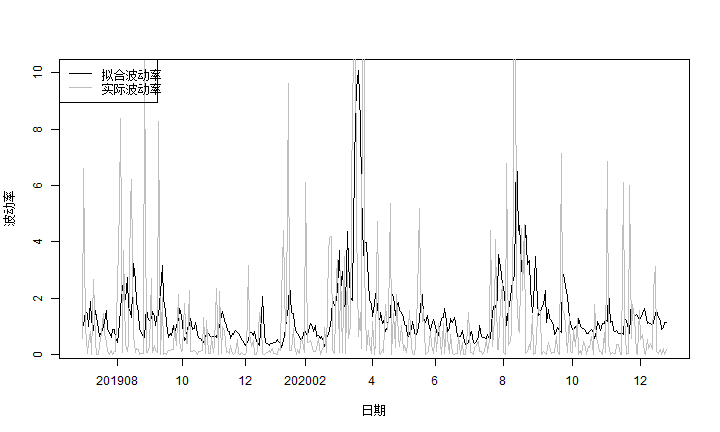
\includegraphics[width=0.95\linewidth]{03-estimation-lytfinal_files/figure-latex/Auvol-1} 

}

\caption{Au(T+D)波动率拟合图}\label{fig:Auvol}
\end{figure}

利用最优模型对Au(T+D)波动率进行拟合,结果如图\ref{fig:Auvol}所示。通过对不同时刻波动率的表现特征分析发现,自2019年8月到9月初,Au(T+D)出现较小幅度的波动,在
2019年7月底-8月初英国强硬脱欧、贸易战愈演愈烈,边缘战争不断爆发等事件的发生点燃了黄金行情。2019年8月以来许多货币对美元出现了贬值,美债收益率倒挂严重,在美国实际利率下行趋势开启的背景下,投资者对经济衰退的担忧加剧,由于黄金具有套期保值的特性,黄金价格逐渐上涨。2020年3月开始Au(T+D)出现了剧烈波动,结合当时现实背景可知,当时新冠疫情在世界大面积爆发,美国、英国等国家逐渐出现疫情失控的局面,市场持悲观态度,市场风险有所增加,这也引起了黄金价格的大幅度上涨,引起了剧烈波动。2020年
8-9月,各国开始陆陆续续公布新冠疫苗的进展,市场有所回暖,但也在一定程度上造成黄金的下跌,其对应的收益率也波动剧烈。

\hypertarget{section-20}{%
\section{结论与启示}\label{section-20}}

本文选取了在贵金属市场中具有代表性的黄金作为研究对象,以Au(T+D)的5分钟高频收益率序列,结合已实现测度RV构建一元Realized GARCH模型,对黄金波动特征研究分析,可获得如下结论:

\begin{enumerate}
\def\labelenumi{\arabic{enumi}.}
\item
  Au(T+D)的收益率序列呈尖峰厚尾的现象,不具有正态分布的特征,且存在显著的条件异方差效应,即在贵金属现货市场中黄金的波动表现出显著的时变性和集聚性。
\item
  利用5分钟高频收益率计算Au(T+D)的已实现方差RV,基于不同分布构建的一元Realized
  GARCH模型后,发现Au(T+D)基于RV和广义双曲线分布的Realized GARCH拟合效果最好,说明已实现方差RV能捕捉到连续的价格突变,减少高频交易数据的微观噪音。
\item
  根据测量方程中的杠杆函数\(\tau(z_{t})\)所对应的\(\tau_1<0\),\(\tau_2>0\),得出收益率序列存在明显的非对称性,即杠杆效应,并且负向收益率冲击对波动率的影响要比正向收益率对波动率的影响更大。
\item
  通过分析最优模型刻画的波动率,发现黄金在市场动荡以及新冠疫情影响下波动剧烈,在市场动荡,趋于不利背景下,贵金属的保值避险优势尽显。
\end{enumerate}




\bibliography{./Bibfile.bib}




\end{document}
